\section{Explicar problema}
\begin{figure}[h]
\centering
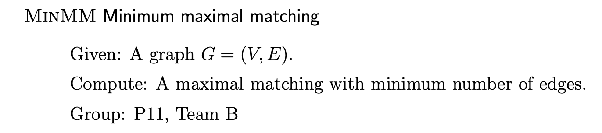
\includegraphics[width=0.8\linewidth]{images/image1.png}
\end{figure}
((A \textbf{maximal matching} is a matching \textit{M} of a graph \textit{G} that is not a subset of any other matching. A matching \textit{M} of a graph \textit{G} is maximal if every edge in \textit{G} has a non-empty intersection with at least one edge in \textit{M}. The following figure shows examples of maximal matchings (red) in three graphs.))

Un \textbf{maximal matching} és un matching M d'un graf G que no és un subset de cap altre matching. Un matching M d'un graf G és maximal si cada aresta en G té una intersecció no buida amb com a mínim una aresta de M. La següent figura mostra matchings maximals (vermell) en tres grafs [1]:
\begin{figure}[h]
\centering
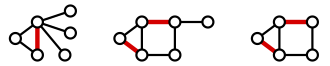
\includegraphics[width=0.8\linewidth]{images/image2.png}
\end{figure}

Un minimal maximal matching és un matching M de G tal que no hi ha cap altre matching amb menor nombre d'arestes.

Propietats:

Un maximal matching M de tamany k per a un graf G és també un edge dominating set de tamany k per a G.
Un edge dominating set és per a un graf G un subset D de les arestes tal que cada aresta fora de D és adjacent a una aresta en D. [2]
\begin{figure}[h]
\centering
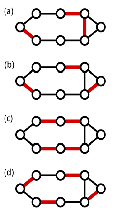
\includegraphics[width=0.8\linewidth]{images/image3.png}
\end{figure}
Busquem minimitzar-ho, per tant, obtenir el conjunt D de mida k mínima tq es forma un dominating set. No hi haura cap subconjunt D de mida k-1 tq siqui un maximal matching, i tota aresta no pertanyent a D sigui adjaceny a una aresta en D.
El problema decisional de trobar un dominating set de tamany k és equivalent al de trobar un maximal matching de tamany k. Aquest problema és també un problema conegut per ser NP-Complet, i la seva versió de minimització NP-Dificil. L'equivalència d'aquests dos problemes ens ajuda a reforçar la complexitat de minimum maximal matching.
